\documentclass{article}

% Using the package for importing pictures.
\usepackage{graphicx}
\graphicspath{{./images/}}

% Configure the paragraph spacing and indentation.
\usepackage{parskip}

% Configuring the margins.
\usepackage[top=25mm, bottom=25mm, left=20mm, right=20mm]{geometry}

% Configuring the headers and footers.
\usepackage{fancyhdr}
\pagestyle{fancy}
\lhead{Developer's Society}
\chead{Coding 101}
\rhead{Jeopardy}

% This package is used to align the name, upi, team on the front
% cover of the report.
\usepackage{varwidth}

\begin{document}
    \section*{Coding 101 Exercise Instructions}
        To build the Jeopardy game, you are going to be writing a couple of functions in the empty \texttt{exercise.js} file. 
         
        More information is provided below regarding the functions you must write, and the documentation regarding some of the helper functions you can use.

        \vspace{5mm}

        \begin{center}
            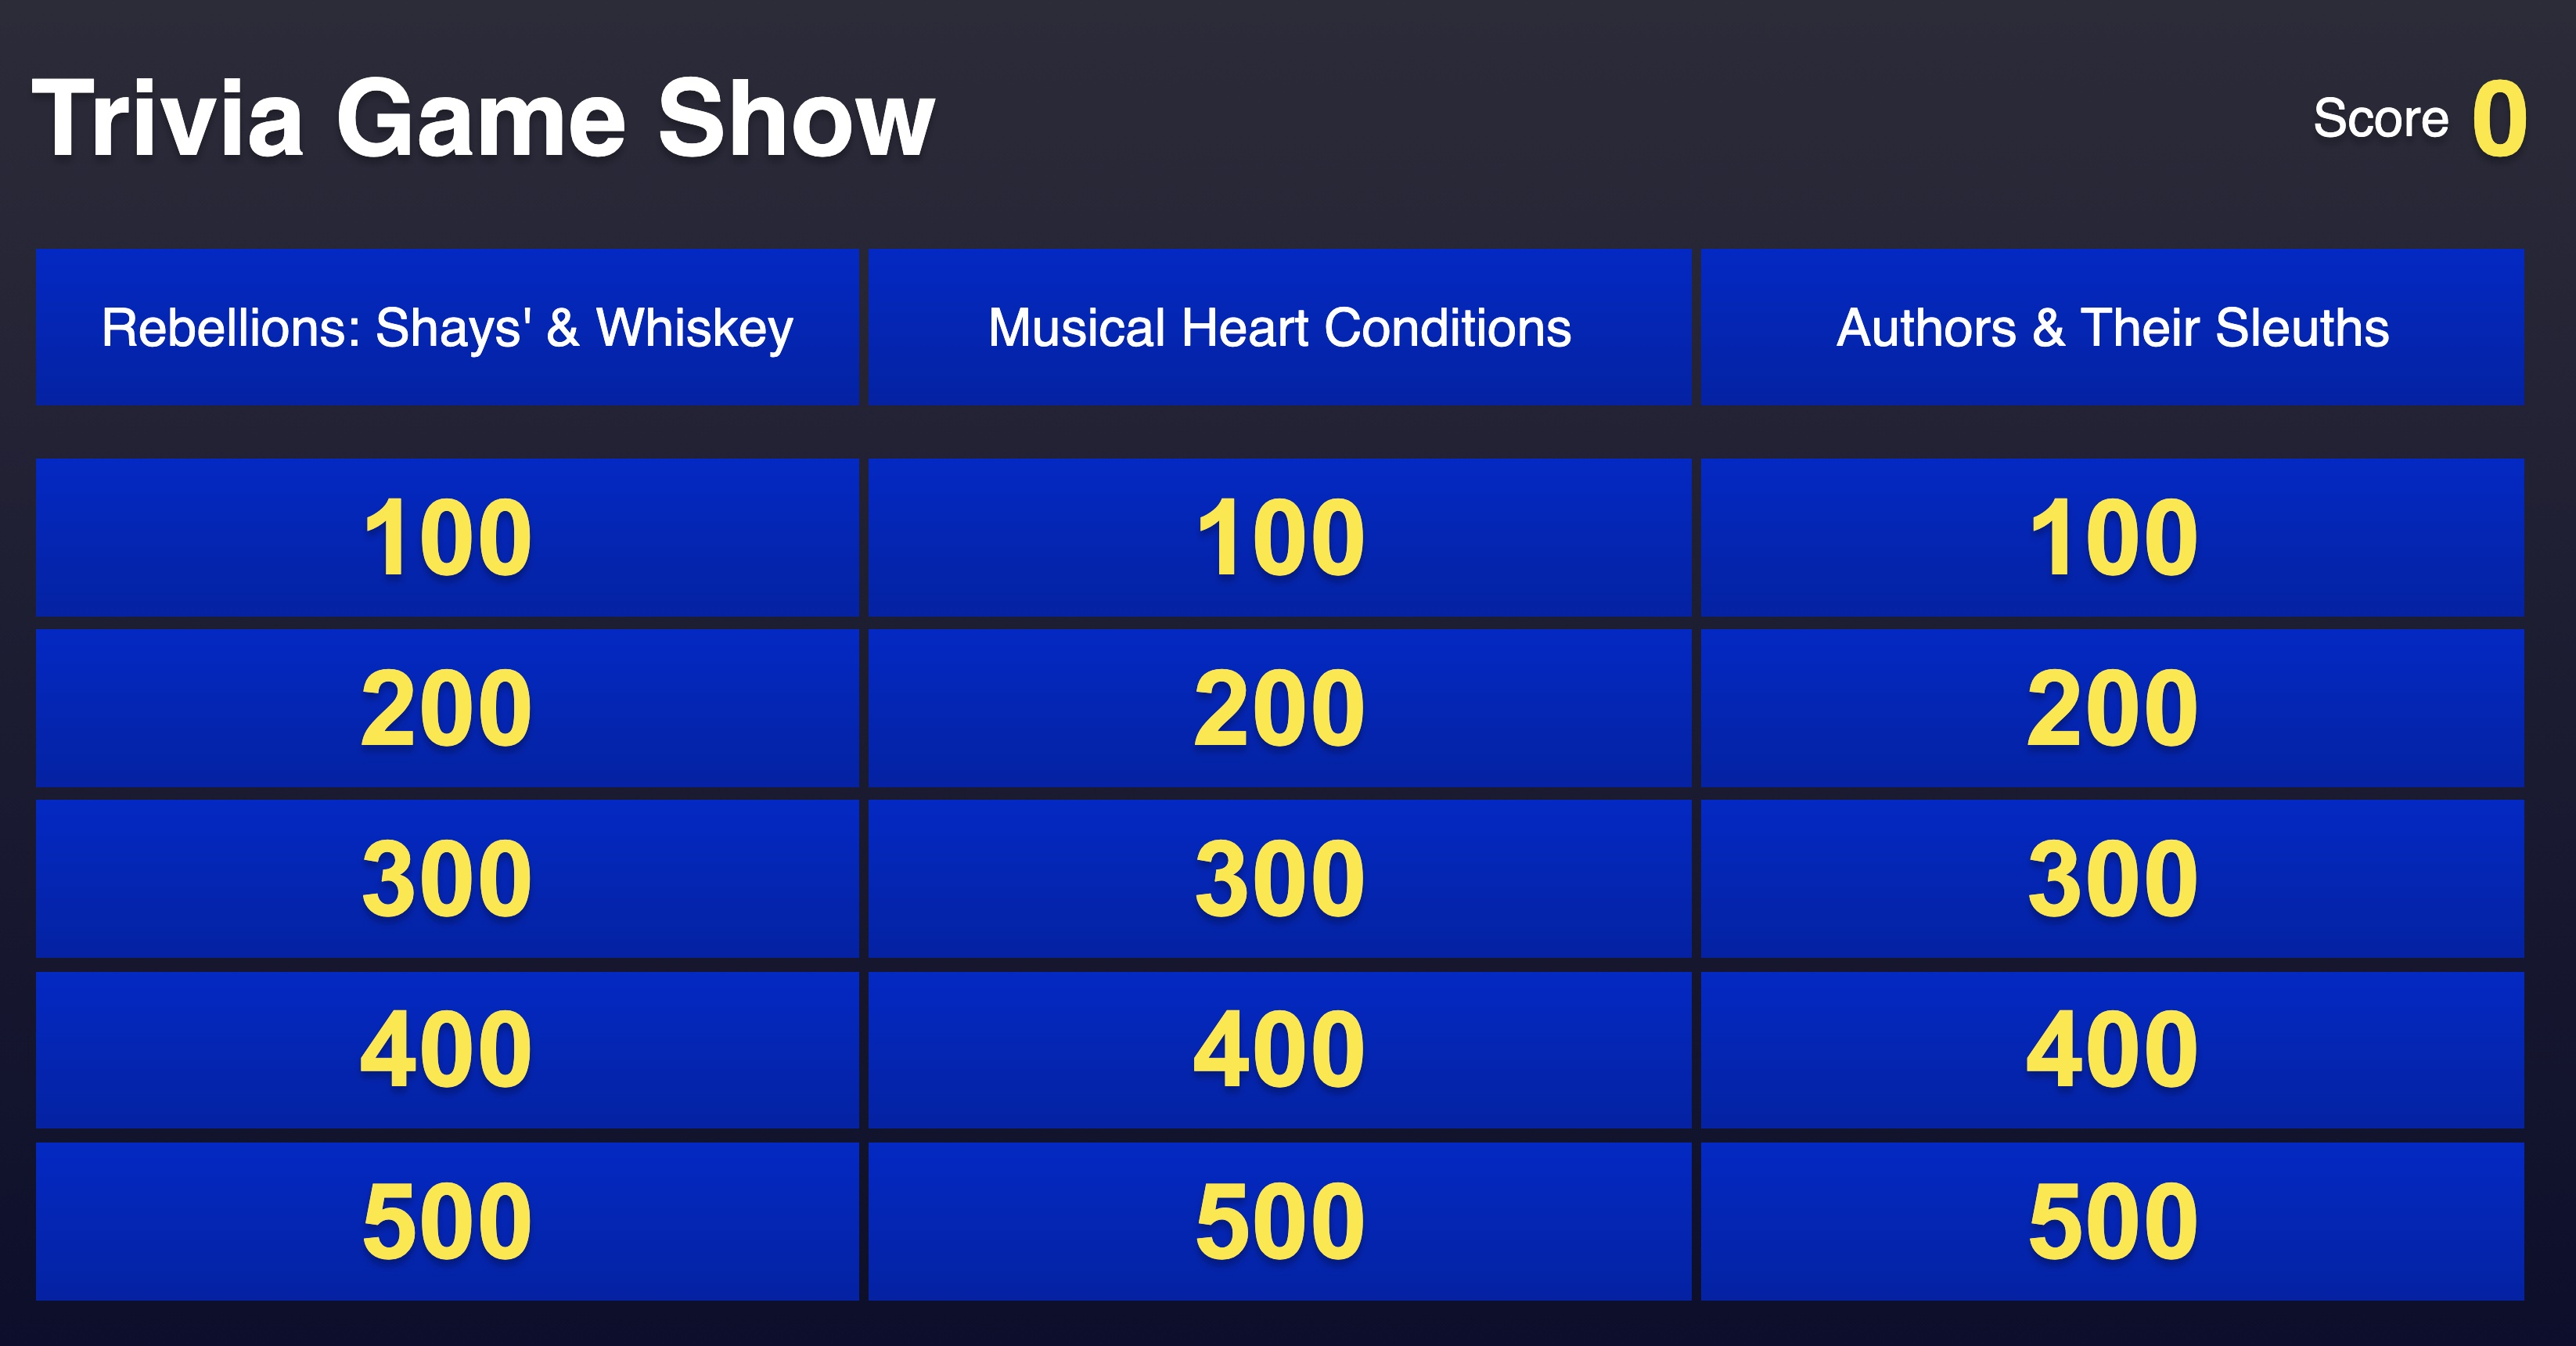
\includegraphics[width=120mm]{jeopardy.jpg}
        \end{center}

    \vspace{5mm}

    \section*{Helper Functions}
        \textbf{Function Name}: \texttt{fetchCategoriesFromAPI} \\
        \textbf{Input(s)}: It only takes a single integer parameter, that specifies the amount of categories you want to request for. \\
        \textbf{Output(s)}: An array containing your requested amount of categories.

        \vspace{3mm}

        \textbf{Function Name}: \texttt{fetchQuestionsFromAPI} \\
        \textbf{Input(s)}: This function takes one parameter, which is the array of the categories you want the questions for. \\
        \textbf{Output(s)}: An array containing all of your questions.
        
        \vspace{3mm}

        \textbf{Function Name}: \texttt{addToGame} \\
        \textbf{Input(s)}: This function takes two parameters. The first parameter is the array of all categories that you got from the helper function. The second parameter is the array of questions for all categories. \\
        \textbf{Output(s)}: This function does not return anything.

    \vspace{5mm}

    \section*{Exercise Instructions}
        \textit{Here is the specification of the functions you will be required to write in the \texttt{exercise.js} file to create the game.}

	\textbf{Function Name}: \texttt{getCategories} \\
        \textbf{Input(s)}: This function takes one parameter, which is the number of categories you'd like to have in the game. \\
        \textbf{Output(s)}: This function should return the array of categories.

        \begin{itemize}
            \item You will need to use one of the helper functions which we have provided, to get the array of categories from the database.
            \item The function will just return this array.
        \end{itemize}

        \textbf{Function Name}: \texttt{getQuestions} \\
        \textbf{Input(s)}: It only takes a single parameter. This parameter is an array of categories that you produced using the function above. \\
        \textbf{Output(s)}: An array containing questions for all categories in the input array. 

        \begin{itemize}
            \item The function should iterate over all categories in the input array, and it should use the \texttt{fetchQuestions} helper function to ask for the questions for each category.
            \item These questions should be stored in an array, which is returned by the function.
        \end{itemize}
\end{document}